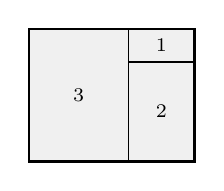
\begin{tikzpicture}[x=0.42cm,y=0.42cm]
\draw[line width=0.5pt,fill=black!6] (0,0) rectangle (3,4);
\node[font=\scriptsize] at (1.5,2.0) {3};
\draw[line width=0.5pt,fill=black!6] (3,0) rectangle (5,3);
\node[font=\scriptsize] at (4.0,1.5) {2};
\draw[line width=0.5pt,fill=black!6] (3,3) rectangle (5,4);
\node[font=\scriptsize] at (4.0,3.5) {1};
\draw[line width=1pt] (0,0) rectangle (5,4);
\end{tikzpicture}\qquad
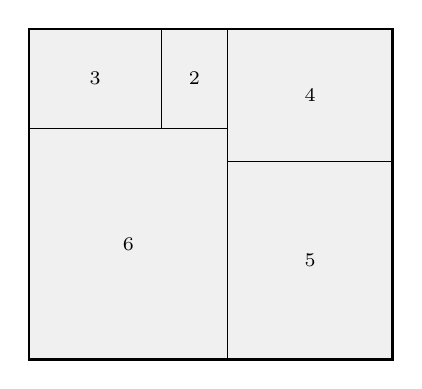
\begin{tikzpicture}[x=0.42cm,y=0.42cm]
\draw[line width=0.5pt,fill=black!6] (0,0) rectangle (6,7);
\node[font=\scriptsize] at (3.0,3.5) {6};
\draw[line width=0.5pt,fill=black!6] (6,0) rectangle (11,6);
\node[font=\scriptsize] at (8.5,3.0) {5};
\draw[line width=0.5pt,fill=black!6] (6,6) rectangle (11,10);
\node[font=\scriptsize] at (8.5,8.0) {4};
\draw[line width=0.5pt,fill=black!6] (0,7) rectangle (4,10);
\node[font=\scriptsize] at (2.0,8.5) {3};
\draw[line width=0.5pt,fill=black!6] (4,7) rectangle (6,10);
\node[font=\scriptsize] at (5.0,8.5) {2};
\draw[line width=1pt] (0,0) rectangle (11,10);
\end{tikzpicture}
